\subsection{Code Verification}
\paragraph{}
We want to check if the code correctly implement the model which has been validated to correctly represent the system. In order ot check it, we look at the event log for a small time interval and verify that the customer's route is followed correctly: arrival, time of queue (if it's necessary), service and checkout from the system.

\begin{figure}[h]
  \begin{center}
  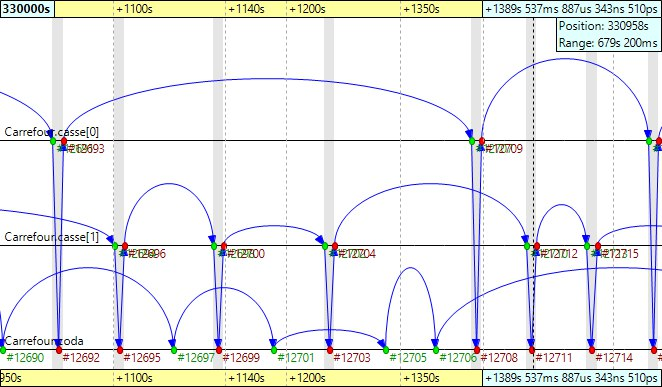
\includegraphics[width=100mm]{elog1.jpg}
  \caption{Single queue eventlog.}
  \label{fig:elogs}
  \end{center}
\end{figure}
\begin{figure}[h]
  \begin{center}
  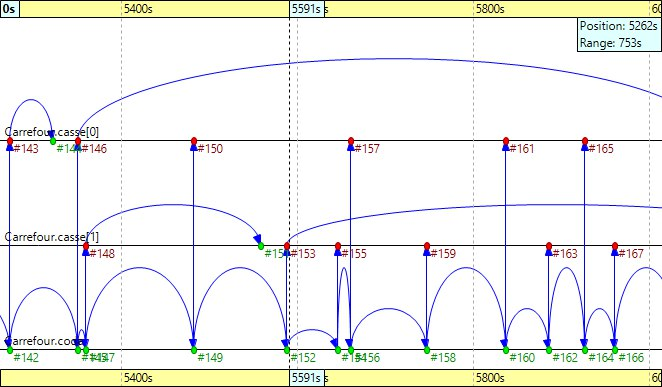
\includegraphics[width=100mm]{elog2.jpg}
  \caption{Multiple queue eventlog.}
  \label{fig:elogm}
  \end{center}
\end{figure}

\paragraph{} Since the system is the steady state, the condition are respected in both cases, single queue and multiple queues, as shown in \ref{fig:elogs} and \ref{fig:elogm}.


